\chapter{Классификация}

\section{Описание подхода}

Предположим, что $Q(x)$, $P(x)$ в уравнении (\ref{eq:stationary}) четные $\pi$-периодические функции.
Определим {\it отображение Пуанкаре} $T: \mathbb{R}^2 \to \mathbb{R}^2$, связанное с уравнением (\ref{eq:stationary}) следующим образом:
%
\begin{equation}
T
\begin{pmatrix}
u_0 \\
u_0'
\end{pmatrix}
=
\begin{pmatrix}
u(\pi) \\
u_x(\pi)
\end{pmatrix},
\end{equation}
%
где $u(x)$ --- решение задачи Коши для уравнения (\ref{eq:stationary}) с начальными условиями
%
\begin{equation}
u(0) = u_0, \quad u_x(0) = u_0'.
\label{eq:initial}
\end{equation}
%
Назовем {\it орбитой} последовательность точек $\{ p_n \}$, $p_n \in \mathbb{R}^2$ (последовательность может быть как конечной, так и бесконечной) такую, что $Tp_n = p_{n+1}$.

Определим множества $\mathcal{U}_L^+, \mathcal{U}_L^- \in \mathbb{R}^2$, $L > 0$ следующим образом: $p = (u_0, u_0') \in \mathcal{U}_L^+$ тогда и только тогда, когда решение задачи Коши для уравнения (\ref{eq:stationary}) с начальными условиями (\ref{eq:initial}) не коллапсирует на промежутке $[0;L]$.
Аналогичным образом определим $\mathcal{U}_L^-$ как множество начальных условий (\ref{eq:initial}) таких, что соответствующее решение задачи Коши для уравнения (\ref{eq:stationary}) не коллапсирует на промежутке $[-L;0]$.
Легко показать, что отображение Пуанкаре $T$ определено только на множестве $\mathcal{U}_{\pi}^+$ и переводит его в множество $\mathcal{U}_{\pi}^-$.
Аналогично, обратное отображение $T^{-1}$ определено только на $\mathcal{U}_{\pi}^-$, и $T \mathcal{U}_{\pi}^- = \mathcal{U}_{\pi}^+$.

Далее, рассмотрим следующую последовательность множеств:
%
\begin{eqnarray*}
&& \Delta_0 = \mathcal{U}_{\pi}^+ \cap \mathcal{U}_{\pi}^-; \\
&& \Delta_{n+1}^+ = T \Delta_n^+ \cap \Delta_0, \quad n = 0,1,\dots; \\
&& \Delta_{n-1}^- = T^{-1} \Delta_n^- \cap \Delta_0, \quad n = 0,1,\dots.
\end{eqnarray*}
%
Очевидно, что $\Delta_0$ состоит из точек, имеющих $T$-образ и $T$-прообраз.
Также верными являются следующие утверждения:
%
\begin{eqnarray*}
&& \{ p \in \Delta_n^+ \} \iff \{ Tp, T^2p, \dots, T^np \in \Delta_0 \}; \\
&& \{ p \in \Delta_n^- \} \iff \{ T^{-1}p, T^{-2}p, \dots, T^{-n}p \in \Delta_0 \}.
\end{eqnarray*}
%
Из этого следует, что множества $\Delta_n^{\pm}$ образуют последовательности по включению вида
%
\begin{eqnarray*}
&& \ldots \subset \Delta_{n+1}^+ \subset \Delta_n^+ \ldots \subset \Delta_1^+ \subset \Delta_0; \\
&& \ldots \subset \Delta_{n+1}^- \subset \Delta_n^- \ldots \subset \Delta_1^- \subset \Delta_0.
\end{eqnarray*}
%
Теперь определим множества $\Delta^{\pm}$ следующим образом:
%
\begin{equation*}
\Delta^+ = \bigcap \limits_{n=1}^{\infty} \Delta_n^+, \quad \Delta^- = \bigcap_{n=1}^{\infty} \Delta_n^-.
\end{equation*}
%
Рассмотрим множество $\Delta = \Delta^+ \cap \Delta^-$.
Оно инвариантно относительно действия отображения $T$.
При этом орбиты, порождаемые точками из $\Delta$, находятся во взаимно-однозначном соответствии с регулярными решениями уравнения (\ref{eq:stationary}).
Аналитическое исследование множеств $\Delta_n^{\pm}$, $\Delta^{\pm}$, $\Delta$ крайне сложно, однако возможно их численное построение.
Такое построение, согласно \cite{AlfAvr}, позволяет предсказать и численно построить решения уравнения (\ref{eq:stationary}).
Главное условие, при котором это оказывается возможным, это то, что <<большая часть>> решений уравнения (\ref{eq:stationary}) должны быть сингулярными.

Утверждения \ref{prop:continuation}, \ref{prop:singular} из предыдущей главы накладывают ограничения на функции $Q(x)$, $P(x)$.
В частности, если $Q(x)$, $P(x)$ ограниченные, периодические, и $P(x) > 0$ $\forall x \in \mathbb{R}$, тогда все решения уравнения (\ref{eq:stationary}) регулярны, и наш подход не может быть применен.
В случае же когда $P(x) < 0$, $Q(x) < 0$, уравнение (\ref{eq:stationary}) не имеет несингулярных решений, за исключением нулевого, следовательно подход также не может быть применен.
Однако, как следует из Утверждения \ref{prop:asymptotic}, если $P(x)$ знакопеременная, то уход на бесконечность в конечной точке является типичным для решений уравнения (\ref{eq:stationary}), и применение нашего подхода для поиска несингулярных решений оправдано.
В работе \cite{AlfAvr} для случая $P(x) \equiv -1$ было показано, что если
%
\begin{itemize}
\item[(а)] множество $\Delta_0$ состоит из конечного числа $N$ компонент связности, $\Delta_0 = \bigcup_{k=1}^N D_k$, причем каждая из компонент $D_k$ является криволинейным четырехугольником, границы которого удовлетворяют специальным условиям гладкости и монотонности \cite{AlfAvr};
\item[(б)] все множества $T D_k \cap D_m$ и $T^{-1} D_k \cap D_m$, $k,m = 1, \dots, N$, непусты, и действие отображения $T$ на кривых, лежащих внутри $D_k$, сохраняет свойства монотонности;
\item[(в)] мера множеств $\Delta_n^{\pm}$ стремиться к нулю при $n \to \infty$; 
\end{itemize}
%
тогда орбиты отображения Пуанкаре $T$, действующего на множестве $\Delta$ находятся во взаимно-однозначном соответствии с бесконечными в обе стороны последовательностями над некоторым алфавитом из $N$ символов.

Этот результат можно пояснить следующим образом.
Пусть символы алфавита --- это числа $1, \dots, N$.
Все компоненты связности множества $\Delta_0$ обозначим за $D_k$, $k = 1, \dots, N$.
Тогда для каждого неколлапсирующего решения $u(x)$ существует единственная орбита $\{ p_k \}$, $k = 0, \pm 1, \pm 2, \dots$, где $p_k \in \Delta$, и соответствующая единственная бесконечная последовательность $\dots, \alpha_{-1}, \alpha_0, \alpha_1, \dots$, $\alpha_k \in \{ 1, \dots, N \}$, такая, что
%
\begin{eqnarray}
\dots, p_{-1} = T^{-1} p_0 \in D_{a_{-1}}, \quad p_0 \in D_{\alpha_0}, \quad p_1 = Tp_0 \in D_{\alpha_1}, \dots
\label{eq:ordits_islands}
\end{eqnarray}
%
Наоборот, для каждой бесконечной (в обе стороны) последовательности чисел $\{ 1, \dots, N \}$ существует единственная орбита ${p_k}$, $k = 0, \pm 1, \pm 2, \dots$, где $p_k \in \Delta$, которая удовлетворяет условию (\ref{eq:ordits_islands}) и соответствует единственному решению $u(x)$.
Проверка условий (а), (б) и (в) в работе \cite{AlfAvr} производилась численно, используя некоторые вспомогательные утверждения.
В результате для уравнения из работы \cite{AlfAvr} была построена полная классификация его регулярных решений.

В следующем разделе мы применим этот подход для случая $U(x) \equiv 0$, т.е., $Q(x) = \omega$, когда линейный потенциал отсутствует, а нелинейный потенциал имеет вид
$$P(x) = \alpha + \cos 2x.$$

\section{Применение: $Q(x) = \omega$, $P(x) = \alpha + \cos 2x$}

В этом разделе мы рассмотрим пример простейшей нелинейной модуляции.
В этом случае уравнение для стационарных состояний имеет вид
%
\begin{equation}
u_{xx} + \omega u + (\alpha + \cos 2x) u^3 = 0.
\label{eq:stationary_obj}
\end{equation}
%

Утверждения 1, 2 накладывают ограничения на параметры $\alpha$, $\omega$.
Так для применения нашего подхода нелинейный потенциал должен быть знакопеременным по пространственной координате $x$, что влечет за собой ограничение $\alpha \in (-1, 1)$.
Другое ограничение, $\omega < 0$, очевидным образом возникает из условия локализации стационарной моды (\ref{eq:localization}).

\paragraph{Множества $\mathcal{U}_{\pi}^{\pm}$.}
Множество $\mathcal{U}_{\pi}^+$ для уравнения (\ref{eq:stationary_obj}) было получено сканированием плоскости $(u,u')$ начальных данных в ходе следующей процедуры.
Задача Коши для уравнения (\ref{eq:stationary_obj}) решалась численно с начальными условиями $u(0) = n \Delta u$, $u_x(0) = m \Delta u'$, $m, n = -L, \dots, L$, где шаги сетки $\Delta u$, $\Delta u'$ выбирались достаточно малыми (типичными значениями были $\Delta u = \Delta u' = 0.01$).
Если абсолютное значение решения задачи Коши на интервале $[0; \pi]$ превышало некоторую достаточно большую величину $u_\infty$, полагалось, что имеет место коллапс решения.
Соответствующая точка помечалась белым цветом.
В противном случае, если на промежутке $[0; \pi]$ коллапса не наблюдалось, точка помечалась темным цветом.
Расчеты были произведены для $u_\infty = 10^5$ и в дальнейшем проверены для $u_\infty = 10^7$.
Результаты расчетов в обоих случаях очень хорошо согласуются друг с другом.
Поскольку уравнение (\ref{eq:stationary_obj}) инвариантно относительно замены $x \to -x$, то множество $\mathcal{U}_{\pi}^-$ есть отражение множества $\mathcal{U}_{\pi}^+$ относительно оси $u$.
Результаты численного эксперимента позволяют нам заключить, что для $\alpha \in (-1, 1)$, множества $\mathcal{U}_{\pi}^{\pm}$ представляют собой {\it неограниченные спирали с бесконечным числом оборотов вокруг начала координат}, см. Рис. \ref{pic:spirals}.
%
\begin{figure}
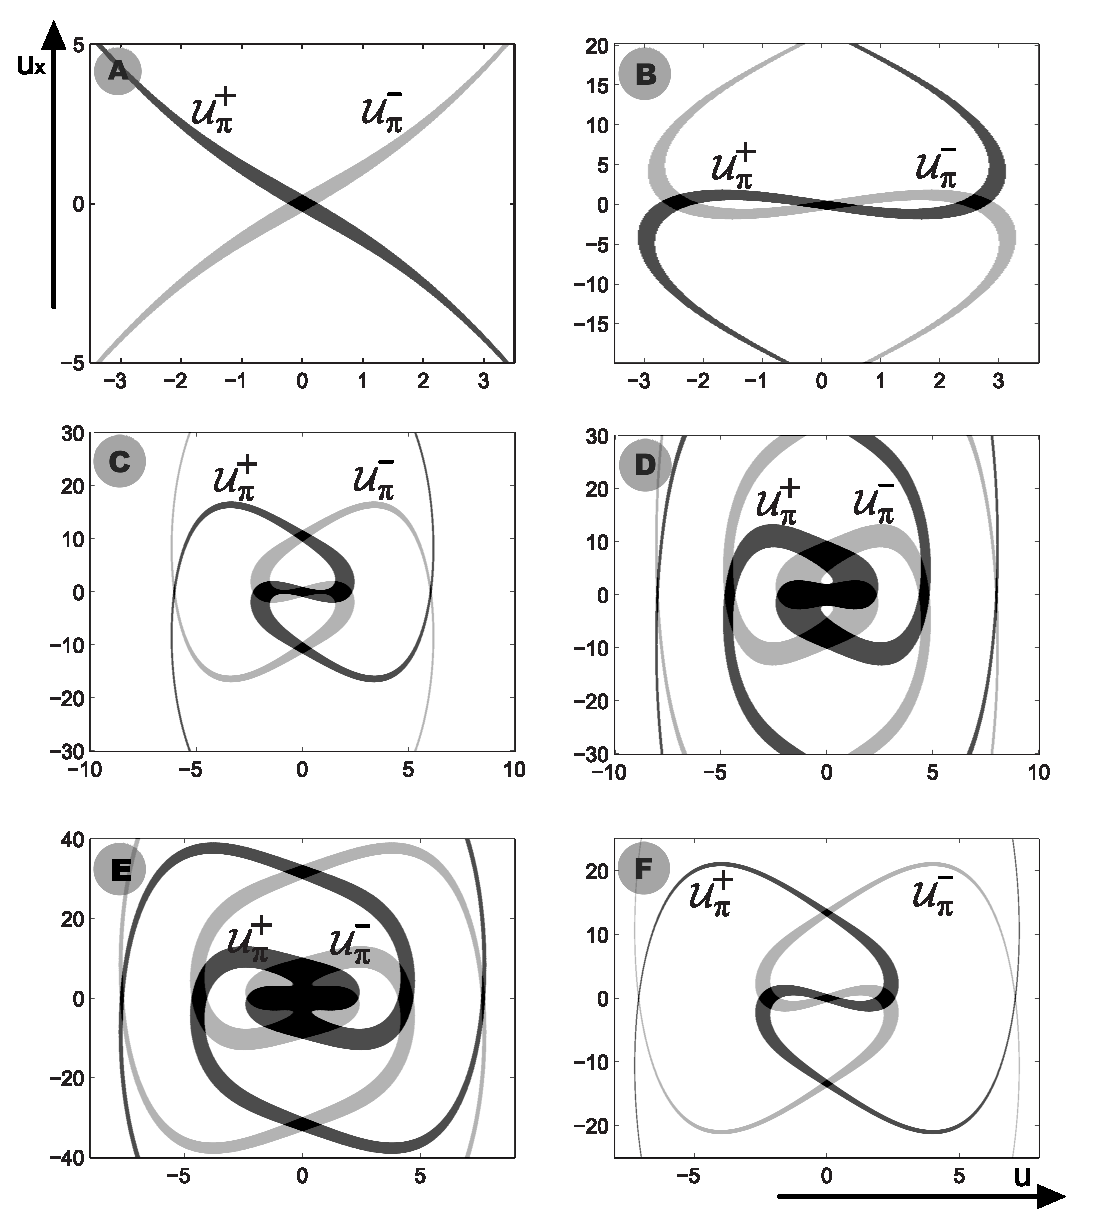
\includegraphics[width=\linewidth]{pic/spirals.eps}
\caption{$\mathcal{U}_{\pi}^{+}$ (темно-серый цвет), $\mathcal{U}_{\pi}^{-}$ (светло-серый цвет) и их пересечение $\Delta_{0}$ для уравнения (\ref{eq:stationary_obj}), при различных значениях параметров $\omega$ и $\alpha$: (A) $\omega = -1$, $\alpha = -1.1$; (B) $\omega = -1$, $\alpha = -0.3$; (C) $\omega = -1$, $\alpha = 0.15$; (D) $\omega = -1$, $\alpha = 0.5$; (E) $\omega = -0.7$, $\alpha = 0.55$; (F) $\omega = -1.5$, $\alpha = 0$.}
\label{pic:spirals}
\end{figure}
%

\paragraph{Множество $\Delta_0$.}
Некоторые примеры множества $\Delta_0$ показаны на Рис. \ref{pic:spirals}.
Рис \ref{pic:spirals} (A) соответствует случаю $\omega = -1$, $\alpha = -1.1$, когда $\Delta_0$ состоит лишь из одной компоненты связности, расположенной в центре координат.
Этот факт согласуется с Утверждением (\ref{prop:singular}).
Орбита единственного в этом случае несинуглярного решения состоит из нулевых точек $p_k = (0, 0)$, каждая из которых принадлежит центральной компоненте связности.
В случае $\alpha \in (-1; 1)$, предположительно, множество $\Delta_0$ неограниченно и состоит из бесконечного числа компонент связности, расположенных вдоль осей $u$ и $u'$, Рис. \ref{pic:spirals} (B)-(F).
Компоненты связности могут быть обозначены символами $\{ A_k \}$, $k = \pm 1, \pm 2, \dots$ (компоненты вдоль оси $u$) и $\{ B_k \}$, $k = \pm 1, \pm 2, \dots$ (компоненты вдоль оси $u'$).
Центральную компоненты связности мы обозначим за $O$.
Основное предположение, важное для применения подхода, заключается в том, что все компоненты связности представляют собой криволинейные четырехугольники, противоположные стороны которых лежат на границах множеств $\mathcal{U}_{\pi}^+$ и $\mathcal{U}_{\pi}^-$.
Исходя из геометрических свойств спирали, естественно полагать, что все компоненты $\{ A_k \}$, $\{ B_k \}$, $k = \pm 1, \pm 2, \dots$ удовлетворяют этому условию.
Однако центральная компонента $O$ может как являться криволинейным четырехугольником, так и не являться им в зависимости от конкретных значений параметров $\omega$, $\alpha$, см. Рис \ref{pic:spirals} и Рис. \ref{pic:central}.
%
\begin{figure}
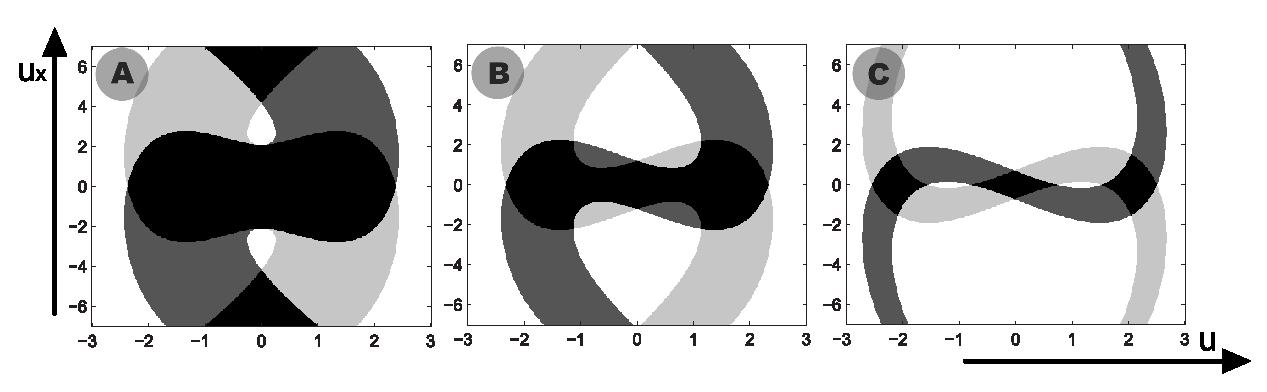
\includegraphics[width=\linewidth]{pic/central.eps}
\caption{Центральная компонента связности $O$ при различных значениях параметров: (A) $\omega = -1$, $\alpha = 0.5$, (B) $\omega = -1$, $\alpha = 0.3$, (C) $\omega = -1$, $\alpha = -0.1$}
\label{pic:central}
\end{figure}
%

\paragraph{Кодирование.}
Предположим, что параметры $\omega$, $\alpha$ таковы, что все компоненты связности в $\Delta_0$ являются криволинейными четырехугольниками.
Тогда численные эксперименты показывают, что $T^{-1} A_k$, $T^{-1} B_k$, $k = \pm 1, \pm 2, \dots$ и $T^{-1} O$ представляют собой бесконечные криволинейные полосы, расположенные внутри множества $\mathcal{U}_{\pi}^+$ и пересекающие все компоненты связности.
Аналогично, $TA_k$, $TB_k$, $k = \pm 1, \pm 2, \dots$ и $TO$ также являются криволинейными полосами, расположенными в $\mathcal{U}_{\pi}^-$, и также пересекают все компоненты связности.
$T$-прообразы множеств
%
\begin{eqnarray*}
& T^{-1} Z \cap A_l, \quad T_{-1} Z \cap B_l, \quad T^{-1} Z \cap O, \quad l = \pm 1, \pm 2, \dots, \\
& Z \in \{ O, A_k, B_k, k = \pm 1, \pm 2, \dots \},
\end{eqnarray*}
%
являются бесконечными криволинейными полосами, принадлежащими $T^{-1} Z$.
Аналогичное утверждение справедливо также для $T$-образов множеств $TZ \cap A_l$, $TZ \cap B_l$, $TZ \cap O$, $l = \pm 1, \pm 2, \dots$, которые находятся внутри $TZ$, где $Z \in \{ O, A_k, B_k, k = \pm 1, \pm 2, \dots \}$.
Таким образом, ситуация оказывается схожей с той, что обсуждалась в работе \cite{AlfAvr}, и мы можем заключить, что динамика отображения $T$ схожа с динамикой соответствующего отображения из \cite{AlfAvr}.
Это, в свою очередь, позволяет нам заключить, что {\it все несингулярные решения уравнения (\ref{eq:stationary_obj}) можно поставить во взаимно-однозначное соответствие с бесконечными в обе стороны последовательностями символов вида $\{ \dots, Z_{-1}, Z_0, Z_1, \dots \}$, где $Z_m \in \{ O, A_k, B_k, k = \pm 1, \pm 2, \dots \}$}.
Орбита, соответствующая коду $\{ \dots, Z_{-1}, Z_0, Z_1 ,\dots\}$, последовательно посещает компоненты связности $Z_m$, $m = \dots, -1, 0, 1, \dots$.
Отметим, что орбита, соответствующая локализованному решению, начинается и заканчивается внутри центральной компоненты связности, следовательно, ей соответствует код вида
%
\begin{equation*}
\{ \dots, O, O, Z_1, Z_2, \dots, Z_n, O, O, \dots \},
\end{equation*}
%
где среди символов символы $Z_1, \dots, Z_m$ есть отличные от $O$.

\paragraph{Солитоны.}
Вне зависимости от того, является ли верным гипотеза о кодировании в случае уравнения (\ref{eq:stationary_obj}), описанный выше подход может быть полезен для предсказания возможных форм стационарных нелинейных мод.
В частности, положение компонент связности множества $\Delta_0$ на плоскости $(u,u')$ и порядок, в котором орбита посещает эти компоненты связности, уже сам по себе несет достаточно много информации о нелинейной моде.
Все рассматриваемые далее солитоны в уравнении (\ref{eq:stationary_obj}) были построены численно, используя прием выхода из линейного приближения.
Некоторые локализованные решения для значений параметров $\omega = -1$, $\alpha = -0.1$ и соответствующие им коды представлены на Рис. \ref{pic:coding}.
%
\begin{figure}
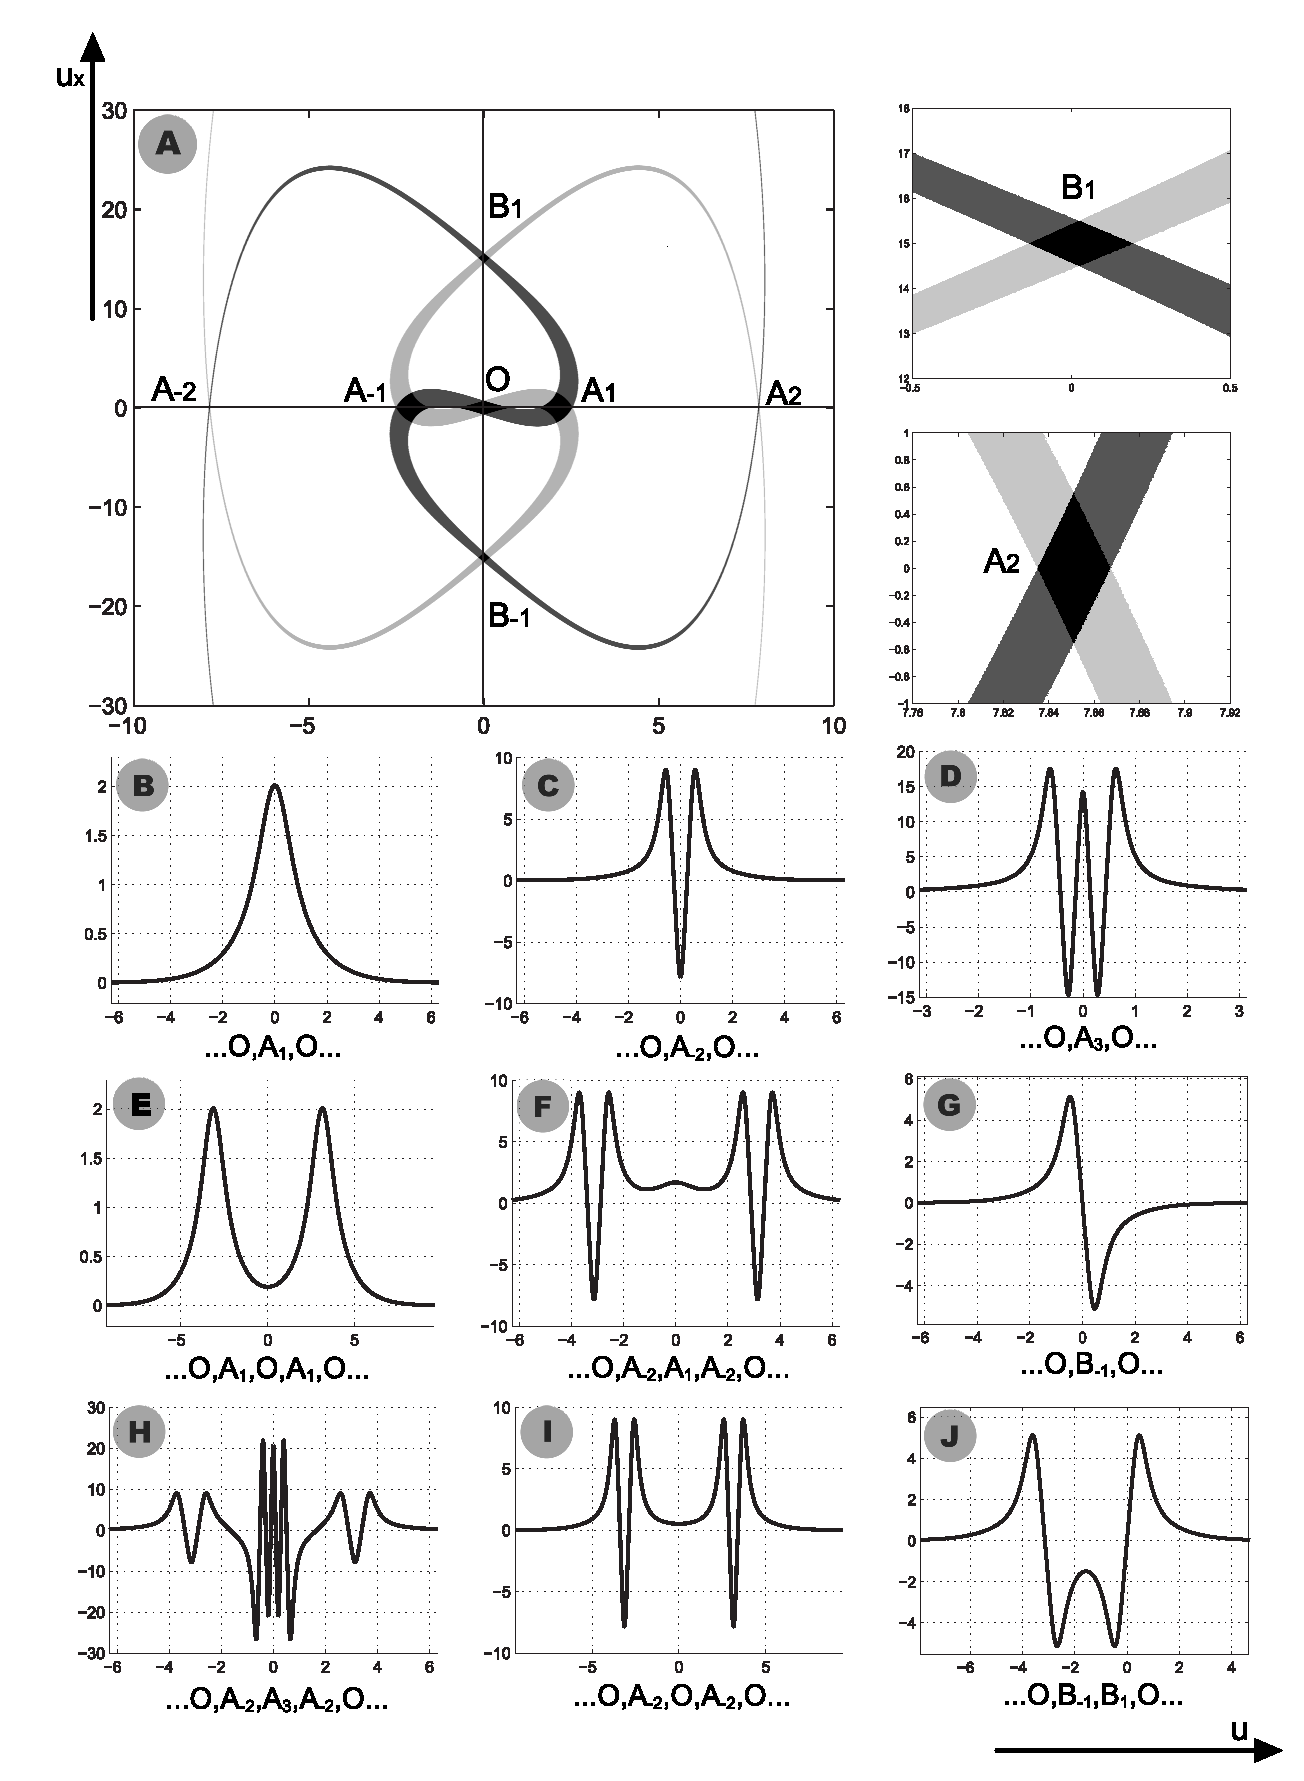
\includegraphics[width=0.92\linewidth]{pic/coding.eps}
\caption{Локализованные решения уравнения (\ref{eq:stationary_obj}) и соответствующие им коды для значений параметров $\omega = -1$, $\alpha = -0.1$; (A) Множества $\mathcal{U}_{\pi}^{\pm}$ и их пересечение $\Delta_0$; (B)-(J) солитоны и их коды}
\label{pic:coding}
\end{figure}
%

Солитон на Рис. \ref{pic:coding} (B) представляет собой фундаментальный солитон (или основной солитон, fundamental soliton, FS) \citep{Malomed}.
Ему соответствует код $\{ \dots, O, A_1, O, \dots \}$, а симметричному относительно оси $u$ солитону соответствует код $\{ \dots, O, A_{-1}, O, \dots \}$.
Другое, важное с физической точки зрения, решение показано на Рис. \ref{pic:coding} (G).
Оно представляет собой так называемый {\it дипольный солитон} (dipole soliton, DS).
Симметричный ему солитон имеет код $\{ \dots, O, B_1, O, \dots \}$.
Это решение аналогично тем, что обсуждались в работах \cite{SFS1}, \cite{SFS2}, \cite{SFS3} при рассмотрении различных вариантов линейного потенциала.
В этих работах похожие классы решений получили название {\it субфундаментальных солитонов} (subfundamental soliton, SFS).
Решения типа DS и SFS объединяет их антисимметричная форма и локализация на одном периоде соответствующей решетки (DS локализован на одном периоде нелинейной решетки, которой соответствует нелинейный потенциал, а SFS, в свою очередь, локализован на одном периоде линейной решетки).

Вообще говоря, стоит отметить, что решение соответствующее коду
%
\begin{equation*}
\{ \dots, O, Z_1, Z_2, \dots, Z_N, O, \dots \},
\end{equation*}
%
где символы $Z_1$ и $Z_N$ отличны от $O$, имеет характерную ширину локализации равную $N\pi$.
Т.е. можно сказать, что такое решение локализовано на $N$ периодах нелинейной решетки.
Например, солитоны, соответствующие кодам $\{ \dots, O, Z, O, \dots \}$, $Z \neq O$, локализованы на одном периоде.
Такие солитоны в дальнейшем мы будем называть {\it элементарными} солитонами.\
Как показывает наш подход, класс локализованных решений уравнения (\ref{eq:stationary_obj}) чрезвычайно широк.
Если наше предположение о бесконечном числе компонент связности множества $\Delta_0$ верно, то уравнение (\ref{eq:stationary_obj}) имеет бесконечное число одних только элементарных солитонов, которые, в свою очередь, могут быть объединены в различные комплексы, как это видно из Рис. \ref{pic:coding}.